%!TEX program = xelatex
\documentclass{beamer}
\usepackage[orientation=landscape,size=custom,width=101.6,height=76.2,scale=1]{beamerposter}

% ---------- packages ----------
\usepackage{fontspec}
\usepackage{graphicx}
\usepackage{tikz}
\usepackage[absolute,overlay]{textpos}

% ---------- font ----------
\setmainfont{GeistMono}[
  Extension      = .ttf,
  UprightFont    = *-Regular,
  BoldFont       = *-Bold,
  ItalicFont     = *-Italic,
  BoldItalicFont = *-BoldItalic,
  Path           = ./fonts/
]
\setsansfont{GeistMono}[
  Extension      = .ttf,
  UprightFont    = *-Regular,
  BoldFont       = *-Bold,
  ItalicFont     = *-Italic,
  Path           = ./fonts/
]
\setmonofont{GeistMono}[
  Extension      = .ttf,
  UprightFont    = *-Regular,
  BoldFont       = *-Bold,
  Path           = ./fonts/
]

% ---------- beamer theme ----------
\usetheme{default}
\usecolortheme{default}
\setbeamertemplate{navigation symbols}{}
\setbeamertemplate{headline}{}
\setbeamertemplate{footline}{}

% White background
\setbeamercolor{background canvas}{bg=white}
\setbeamercolor{normal text}{fg=black}

% ---------- colours ----------
\definecolor{uigold}{HTML}{FFCD00}
\definecolor{uiblack}{HTML}{2C2C2E}

% ---------- kill beamer spacing ----------
\setlength{\parskip}{0pt}
\setlength{\parsep}{0pt}
\setlength{\itemsep}{0pt}
\setlength{\topsep}{0pt}
\linespread{0.82}

% ---------- text position unit ----------
\setlength{\TPHorizModule}{\paperwidth}
\setlength{\TPVertModule}{\paperheight}

% ---------- pill label command ----------
% Usage: \pillhead{Label Text}
\newcommand{\pillhead}[1]{%
  \tikz[baseline=(n.base)]\node[
    fill=uiblack,
    rounded corners=20pt,
    inner xsep=24pt,
    inner ysep=12pt,
  ](n){\textcolor{uigold}{\fontsize{42}{50}\selectfont\bfseries #1}};%
}

% ======================================================================
\begin{document}
\begin{frame}[t]

% ---- dark header band ----
\begin{tikzpicture}[remember picture, overlay]
  \fill[uiblack] (current page.north west)
    rectangle ([yshift=-0.155\paperheight]current page.north east);
\end{tikzpicture}

% ---- gold column dividers ----
\begin{tikzpicture}[remember picture, overlay]
  \draw[uigold, line width=3pt]
    ([xshift=0.335\paperwidth, yshift=-0.155\paperheight]current page.north west)
    -- ([xshift=0.335\paperwidth]current page.south west);
  \draw[uigold, line width=3pt]
    ([xshift=0.667\paperwidth, yshift=-0.155\paperheight]current page.north west)
    -- ([xshift=0.667\paperwidth]current page.south west);
\end{tikzpicture}

% ---- top-left: EXPO logo ----
\begin{textblock}{0.28}(0.02, 0.02)
  
\includegraphics[height=8cm]{expo.png}
\end{textblock}

% ---- top-right: UI Block I logo ----
\begin{textblock}{0.10}(0.91, -0.01)
  
\includegraphics[height=11cm]{uiLogo.png}
\end{textblock}

% ---- bottom-right: College of Engineering logo ----
\begin{textblock}{0.25}(0.91, 0.96)
  
\includegraphics[height=2.4cm]{UIcollegeOfEngLogo.png}
\end{textblock}

% ---- title ----
\begin{textblock}{0.55}(0.25, 0.03)
  {\fontsize{80}{88}\selectfont\bfseries\color{white} TerraCrate}
\end{textblock}

% ---- subtitle ----
\begin{textblock}{0.65}(0.25, 0.075)
  {\fontsize{36}{42}\selectfont\color{uigold} Secure, offline-first file storage for local networks}
\end{textblock}

% ---- authors ----
\begin{textblock}{0.65}(0.25, 0.11)
  {\fontsize{32}{38}\selectfont\color{white} Andreas Neacsu, Adam Cobb, Kevin Ellis, and Devon Bryce}
\end{textblock}

% ==============================================================
% COLUMN 1  (x = 0.02, width = 0.295)
% ==============================================================

% -- Value Proposition --
\begin{textblock}{0.295}(0.02, 0.17)
  \setlength{\baselineskip}{28pt}\setlength{\parskip}{6pt}%
  \pillhead{Value Proposition}\vspace{18pt}\par
  {\fontsize{28}{36}\selectfont\setlength{\baselineskip}{38pt}%
    Existing file-sharing solutions force a trade-off between security and portability.
    USB drives lack access control, commercial NAS requires permanent infrastructure,
    and cloud platforms introduce third-party trust dependencies and internet requirements.
    No lightweight solution combines certificate based authentication, fine-grained access
    control, and zero configuration discovery in a single self contained device.\par}
\end{textblock}

% -- Objective --
\begin{textblock}{0.295}(0.02, 0.37)
  \setlength{\baselineskip}{28pt}\setlength{\parskip}{6pt}%
  \pillhead{Objective}\vspace{18pt}\par
  {\fontsize{28}{36}\selectfont\setlength{\baselineskip}{38pt}%
    Build a portable, self-hosted file server on a Raspberry Pi that provides secure
    multi-user file sharing with mTLS authentication, three-tier permissions, and mDNS
    discovery, deployable in any environment without cloud infrastructure or client
    software beyond a browser.\par}
\end{textblock}

% -- Problem Definition --
\begin{textblock}{0.295}(0.02, 0.52)
  \setlength{\baselineskip}{28pt}\setlength{\parskip}{6pt}%
  \pillhead{Problem Definition}\vspace{18pt}\par
  {\fontsize{28}{36}\selectfont\setlength{\baselineskip}{38pt}%
    TerraCrate gives you full custody of your data in a device you can carry in your
    pocket. Plug it in and it is discoverable. Approve a user and they get a certificate
    in their inbox. Pull the plug and your data goes with you. No cloud, no residue,
    no trust required.\par}
\end{textblock}
\begin{textblock}{0.295}(0.02, 0.67)
  \setlength{\baselineskip}{28pt}\setlength{\parskip}{6pt}%
  \pillhead{Key Requirements}\vspace{18pt}\par
  {\fontsize{28}{36}\selectfont\setlength{\baselineskip}{38pt}%
 All communication must occur over HTTPS, with regular users authenticating via mutual TLS. The system must handle the full certificate lifecycle including generation, delivery via SMTP, and CRL-enforced revocation. A three-tier permission model spanning domain, group, and per-user overrides govern folder access. The device must advertise itself via mDNS with a Wi-Fi AP fallback for infrastructure less environments. All security relevant actions must be recorded in an audit log, and the entire system must run self-contained with no external dependencies.\par}
\end{textblock}

% -- bottom-left images --
\begin{textblock}{0.05}(0, 0.932)
  
\includegraphics[width=\linewidth]{9.PNG}
\end{textblock}
\begin{textblock}{0.05}(0.05, 0.932)
  
\includegraphics[width=\linewidth]{11.PNG}
\end{textblock}
\begin{textblock}{0.05}(0.1, 0.932)
  
\includegraphics[width=\linewidth]{12.PNG}
\end{textblock}

% ==============================================================
% COLUMN 2  (x = 0.352, width = 0.29)
% ==============================================================

\begin{textblock}{0.31}(0.352, 0.17)
  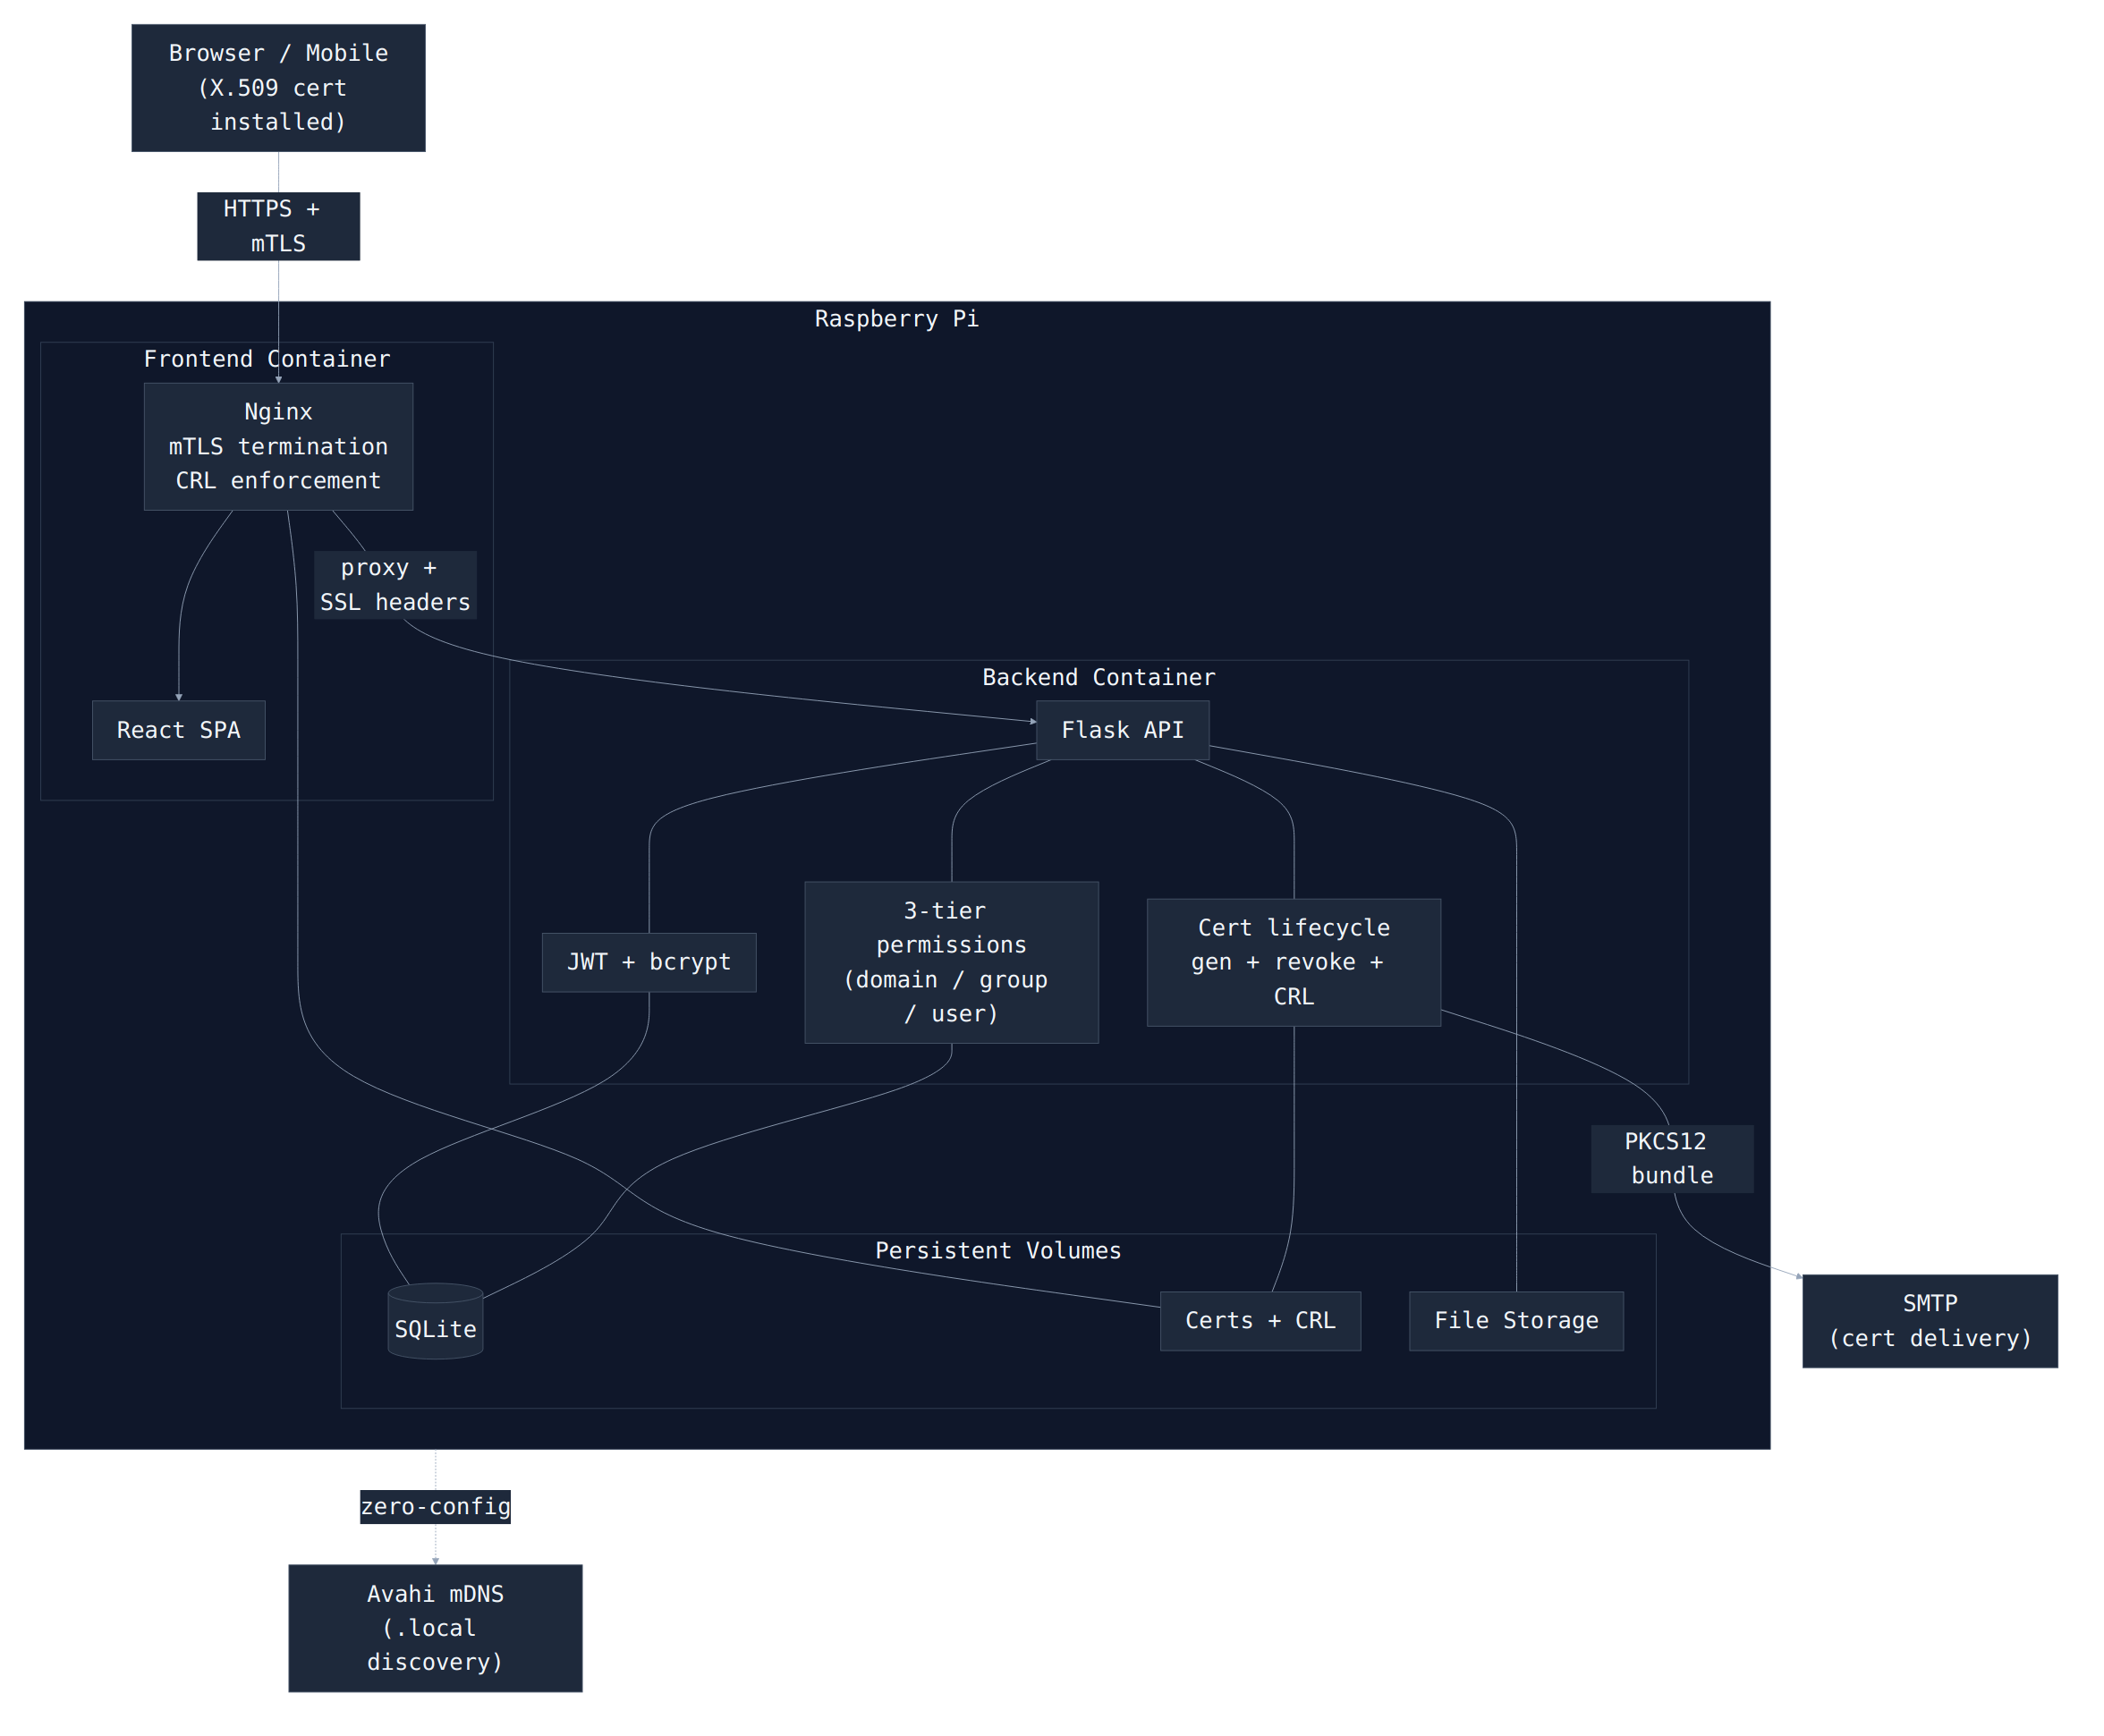
\includegraphics[width=\linewidth]{../diagrams/png/11-sys-arch-slim.png}
\end{textblock}
\begin{textblock}{0.31}(0.352, 0.17)
  \vspace{3pt}\hfill\pillhead{System Architecture}
\end{textblock}

\begin{textblock}{0.31}(0.352, 0.51)
  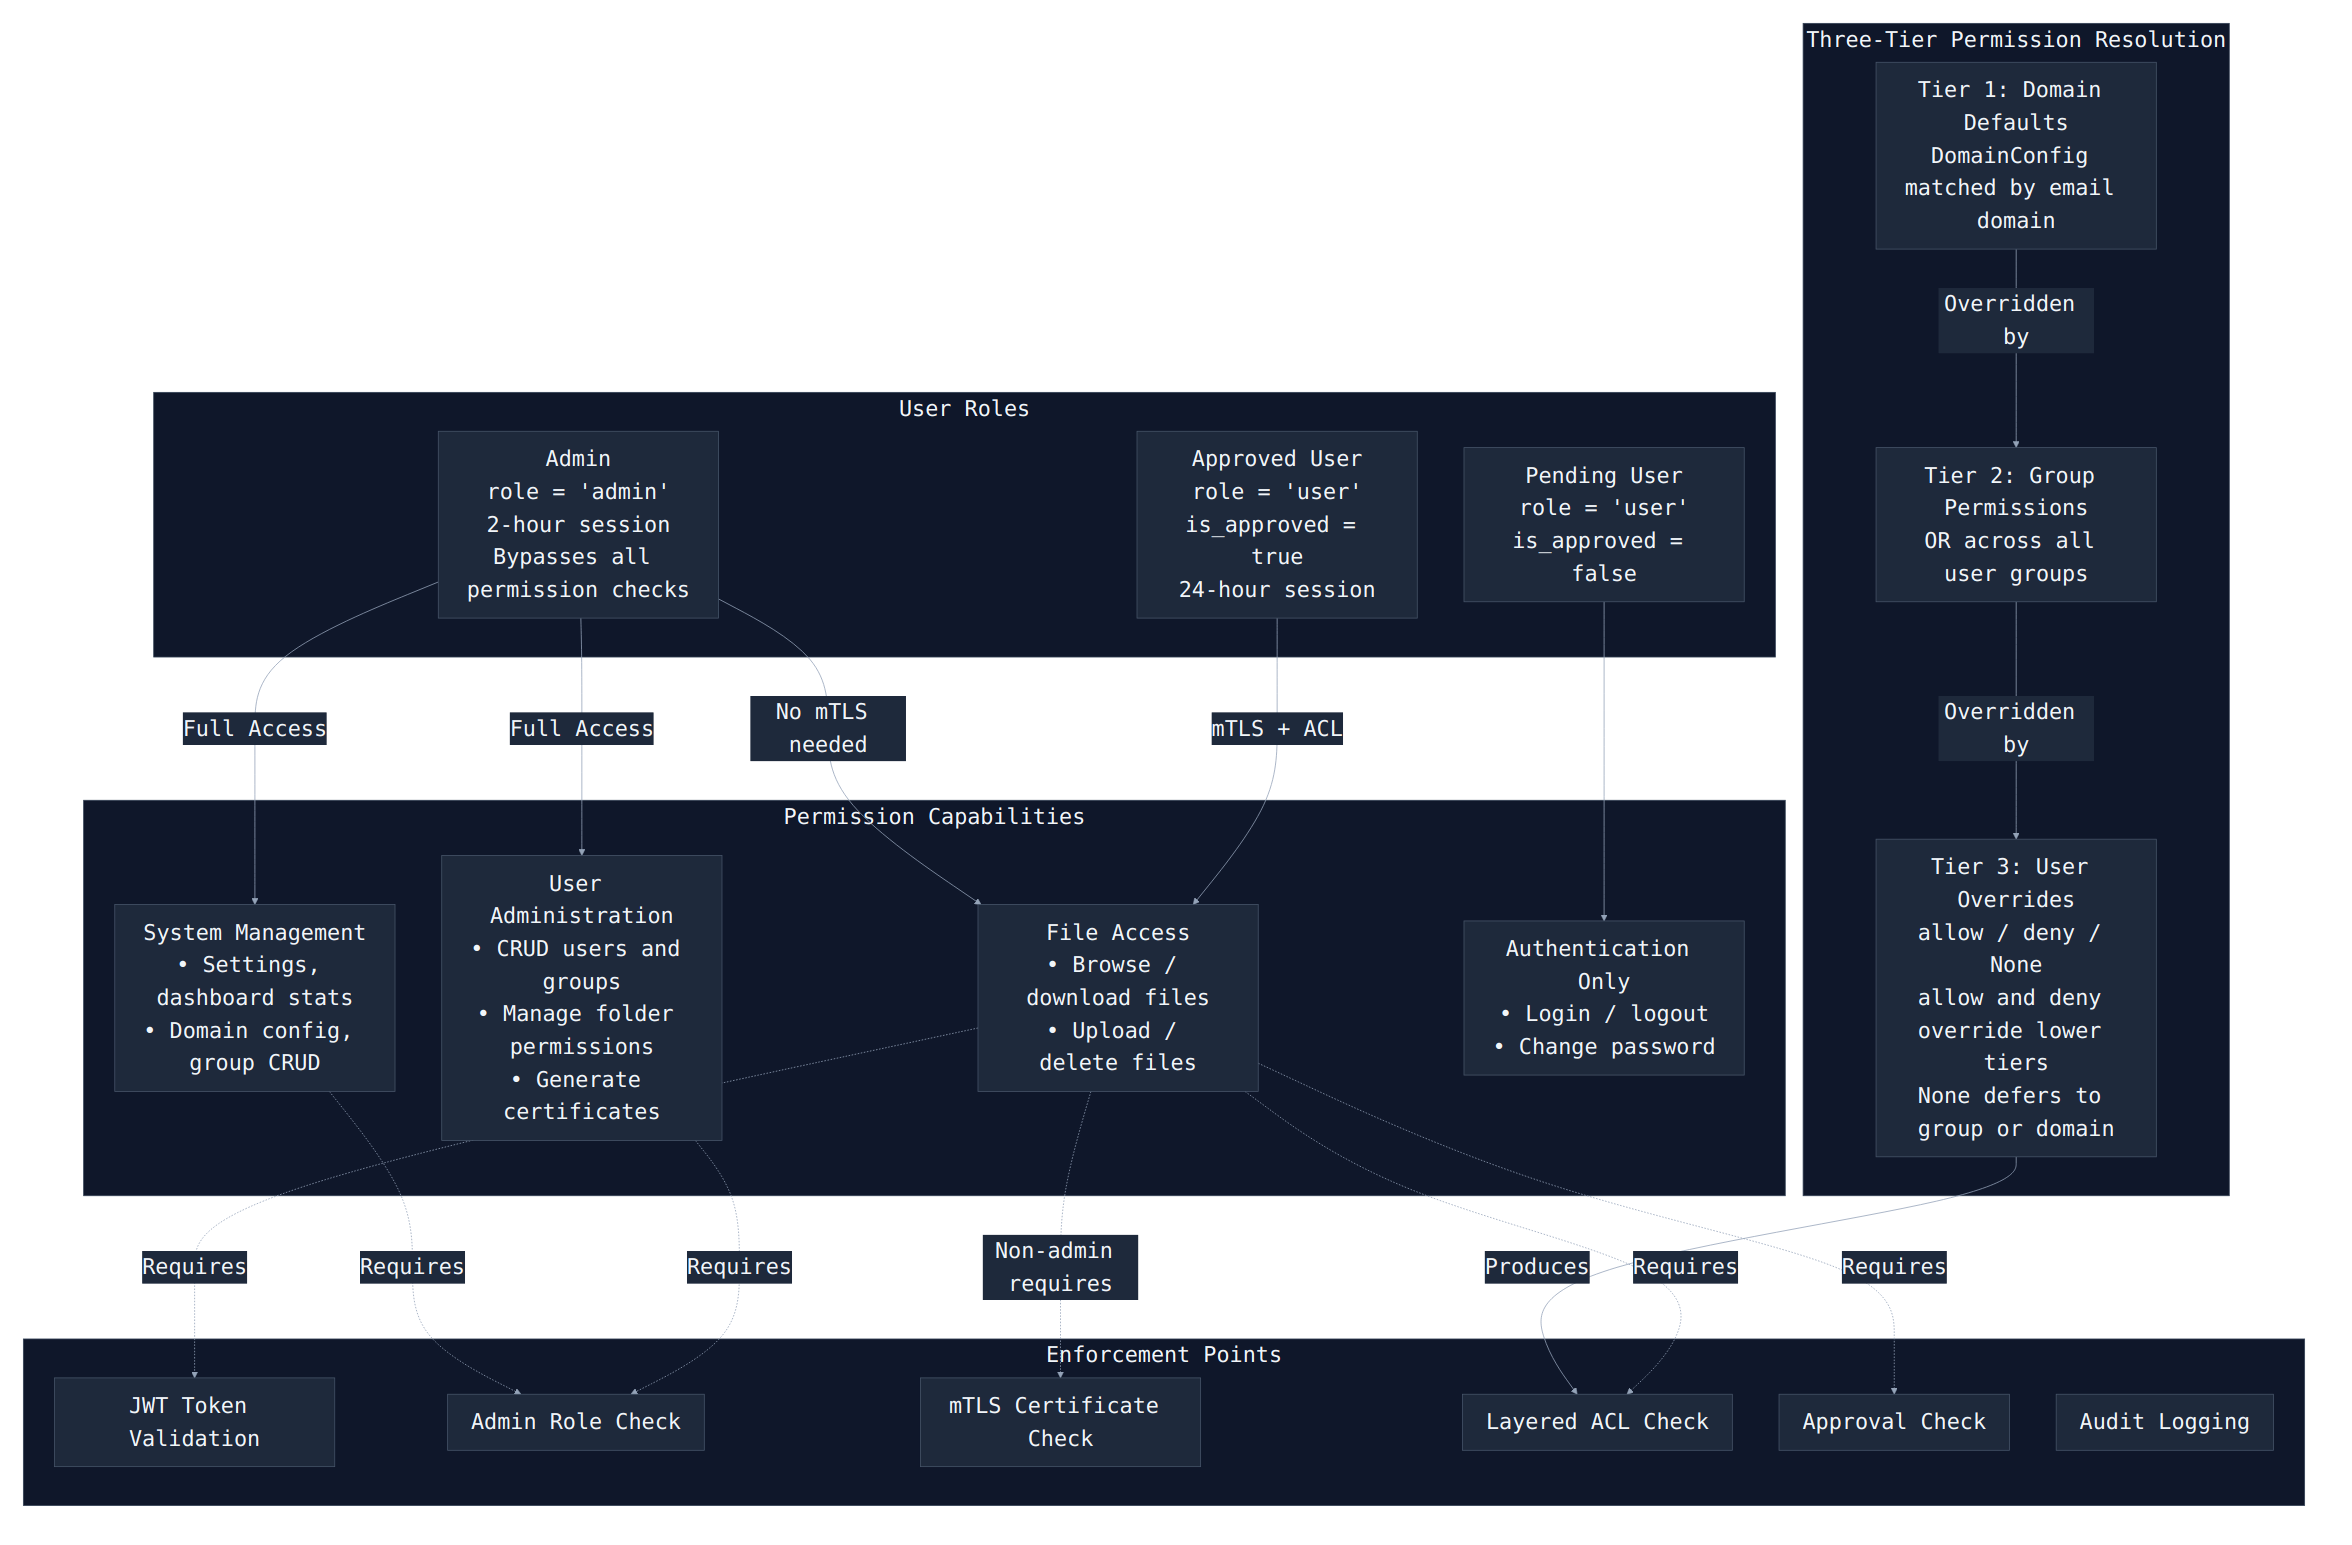
\includegraphics[width=\linewidth]{../diagrams/png/03-rbac.png}
\end{textblock}
\begin{textblock}{0.10}(0.352, 0.54)
  \vspace{3pt}\pillhead{RBAC}
\end{textblock}

% -- Concept Development --
\begin{textblock}{0.31}(0.352, 0.80)
  \setlength{\baselineskip}{28pt}\setlength{\parskip}{6pt}%
  \pillhead{Concept Development}\vspace{18pt}\par
  {\fontsize{28}{36}\selectfont\setlength{\baselineskip}{38pt}%
Two prior designs were evaluated: an SMB-over-mTLS approach requiring client-side Docker, and a QR code JWT approach lacking mutual TLS and per-user access control. The final design resolves both by delegating mTLS verification to Nginx, requiring only a browser with an installed certificate.\par}
\end{textblock}

% ==============================================================
% COLUMN 3  (x = 0.684, width = 0.29)
% ==============================================================

% \begin{textblock}{0.29}(0.684, 0.2)
%   \pillhead{Certificate Revocation}\vspace{3pt}\par
%   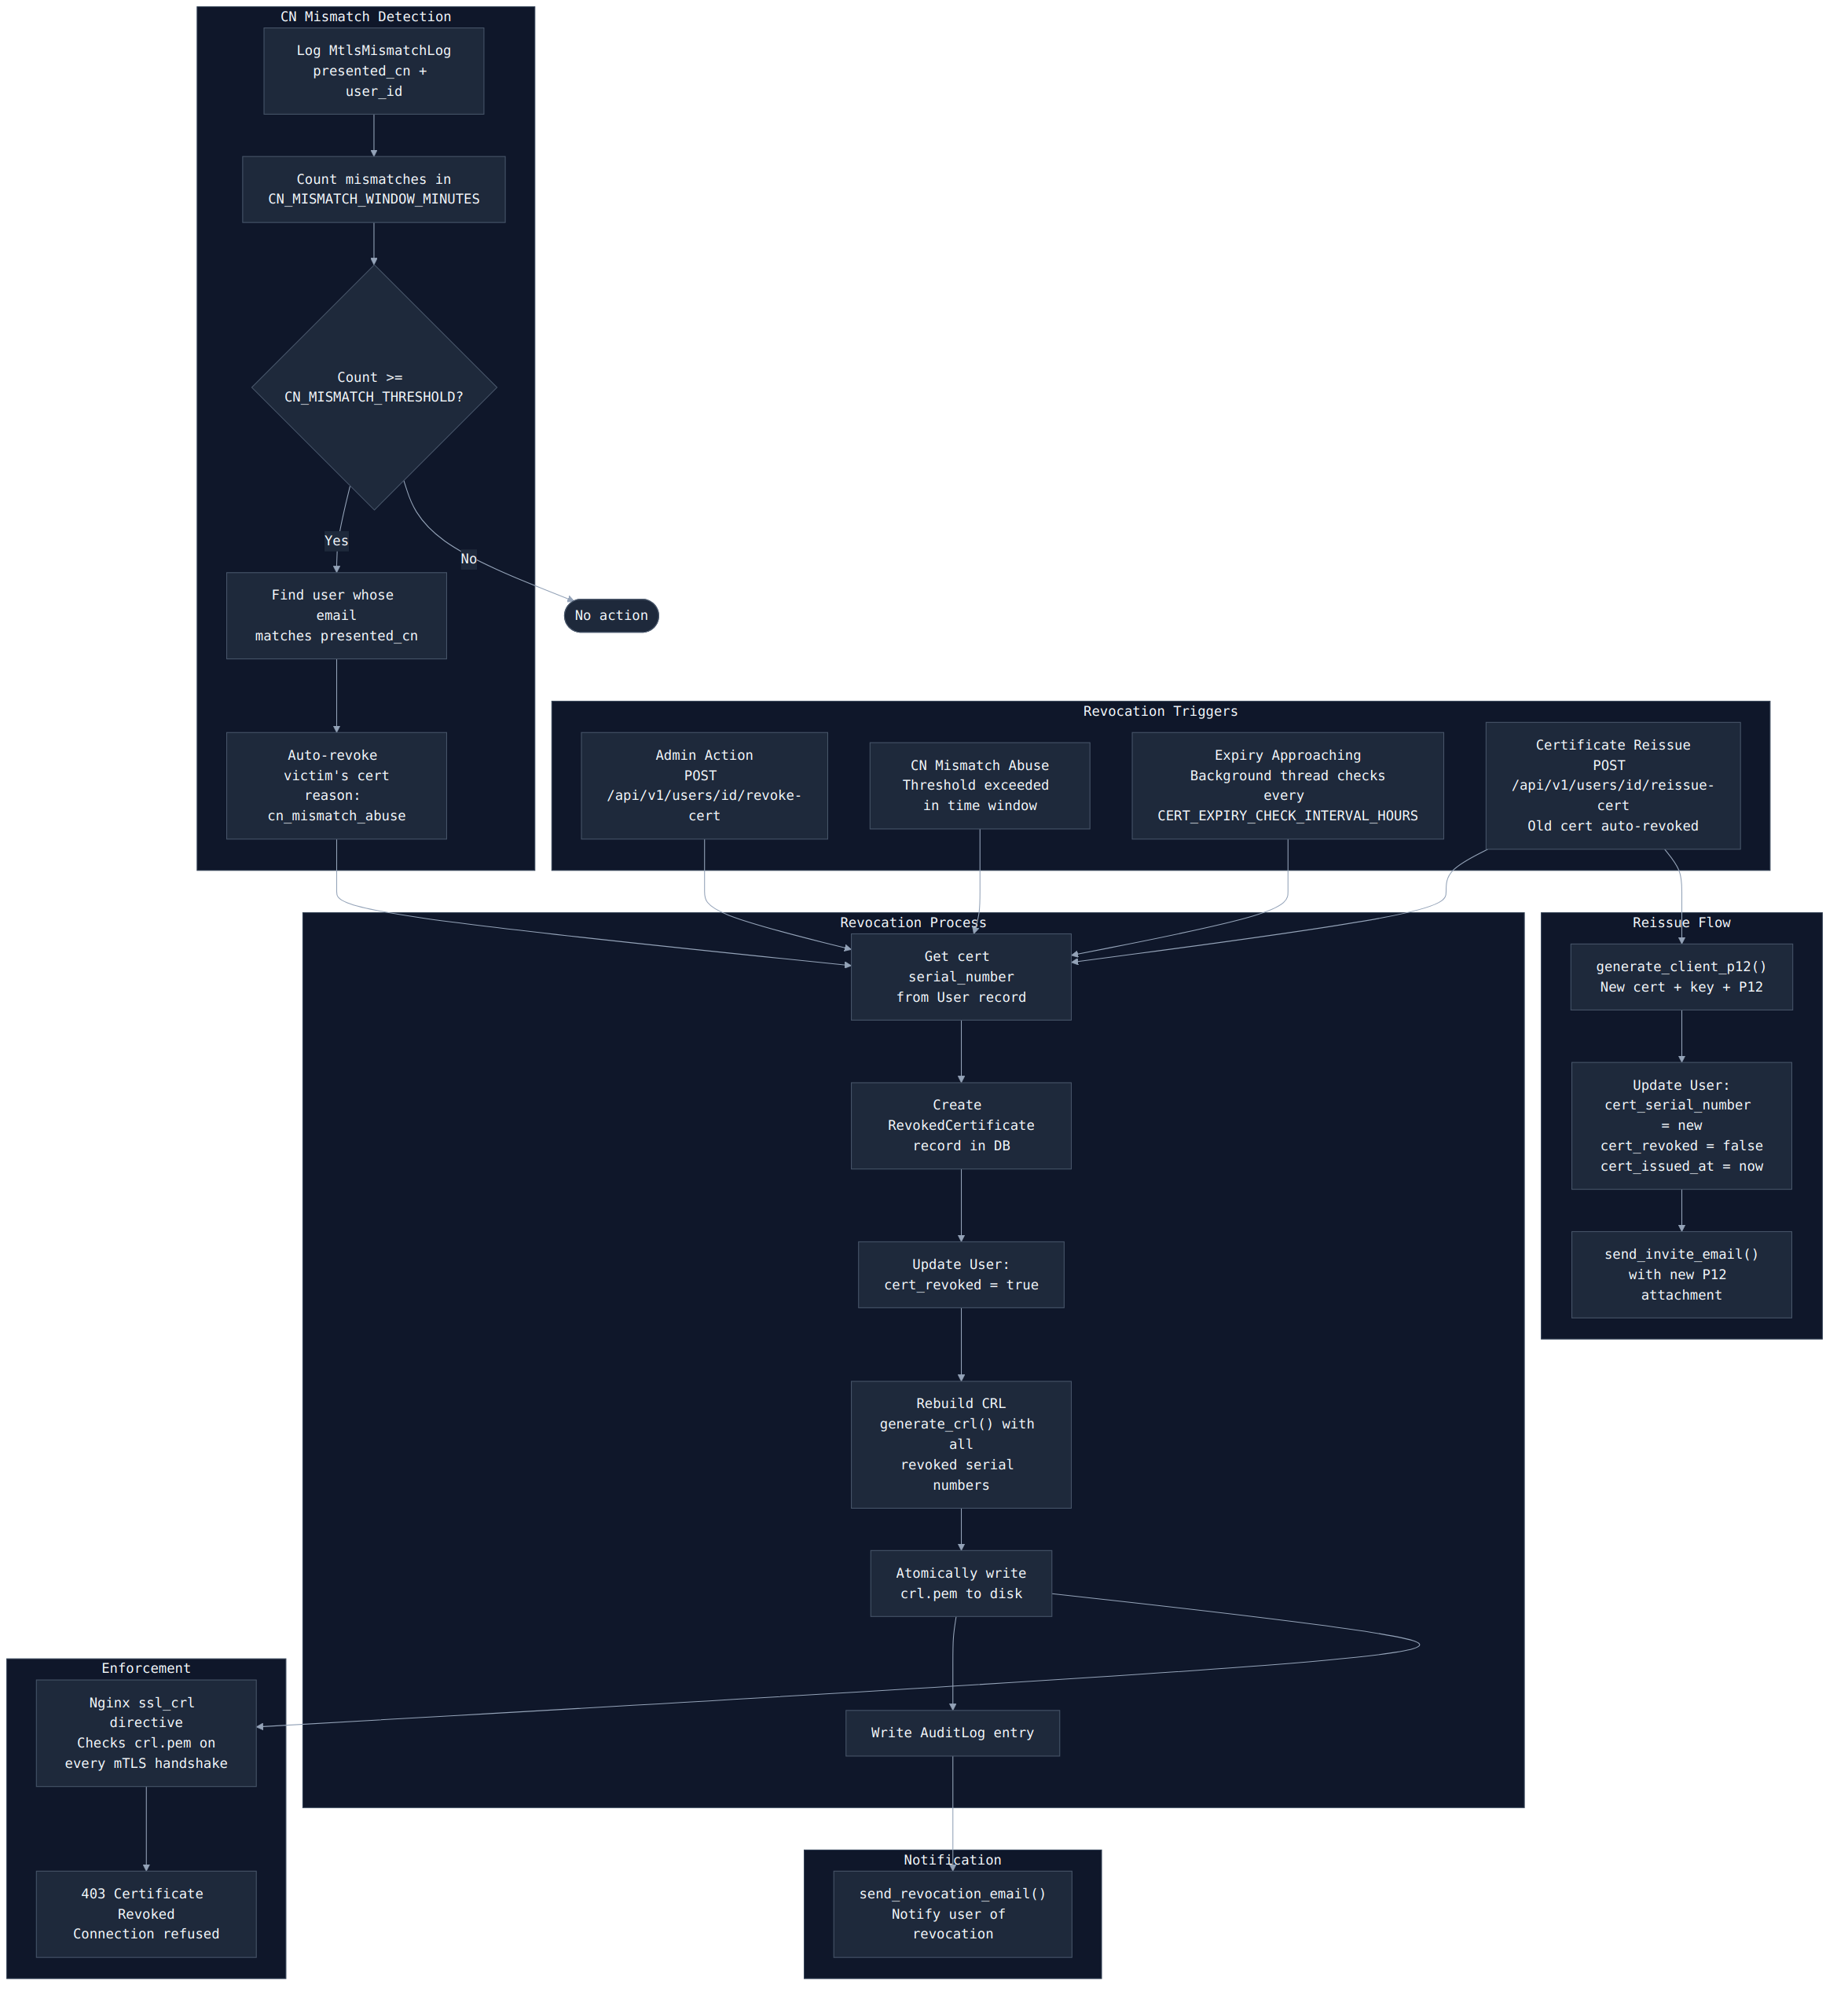
\includegraphics[width=\linewidth]{../diagrams/png/09-certificate-revocation.png}
% \end{textblock}

% \begin{textblock}{0.29}(0.684, 0.54)
%   \pillhead{Audit Logging}\vspace{3pt}\par
%   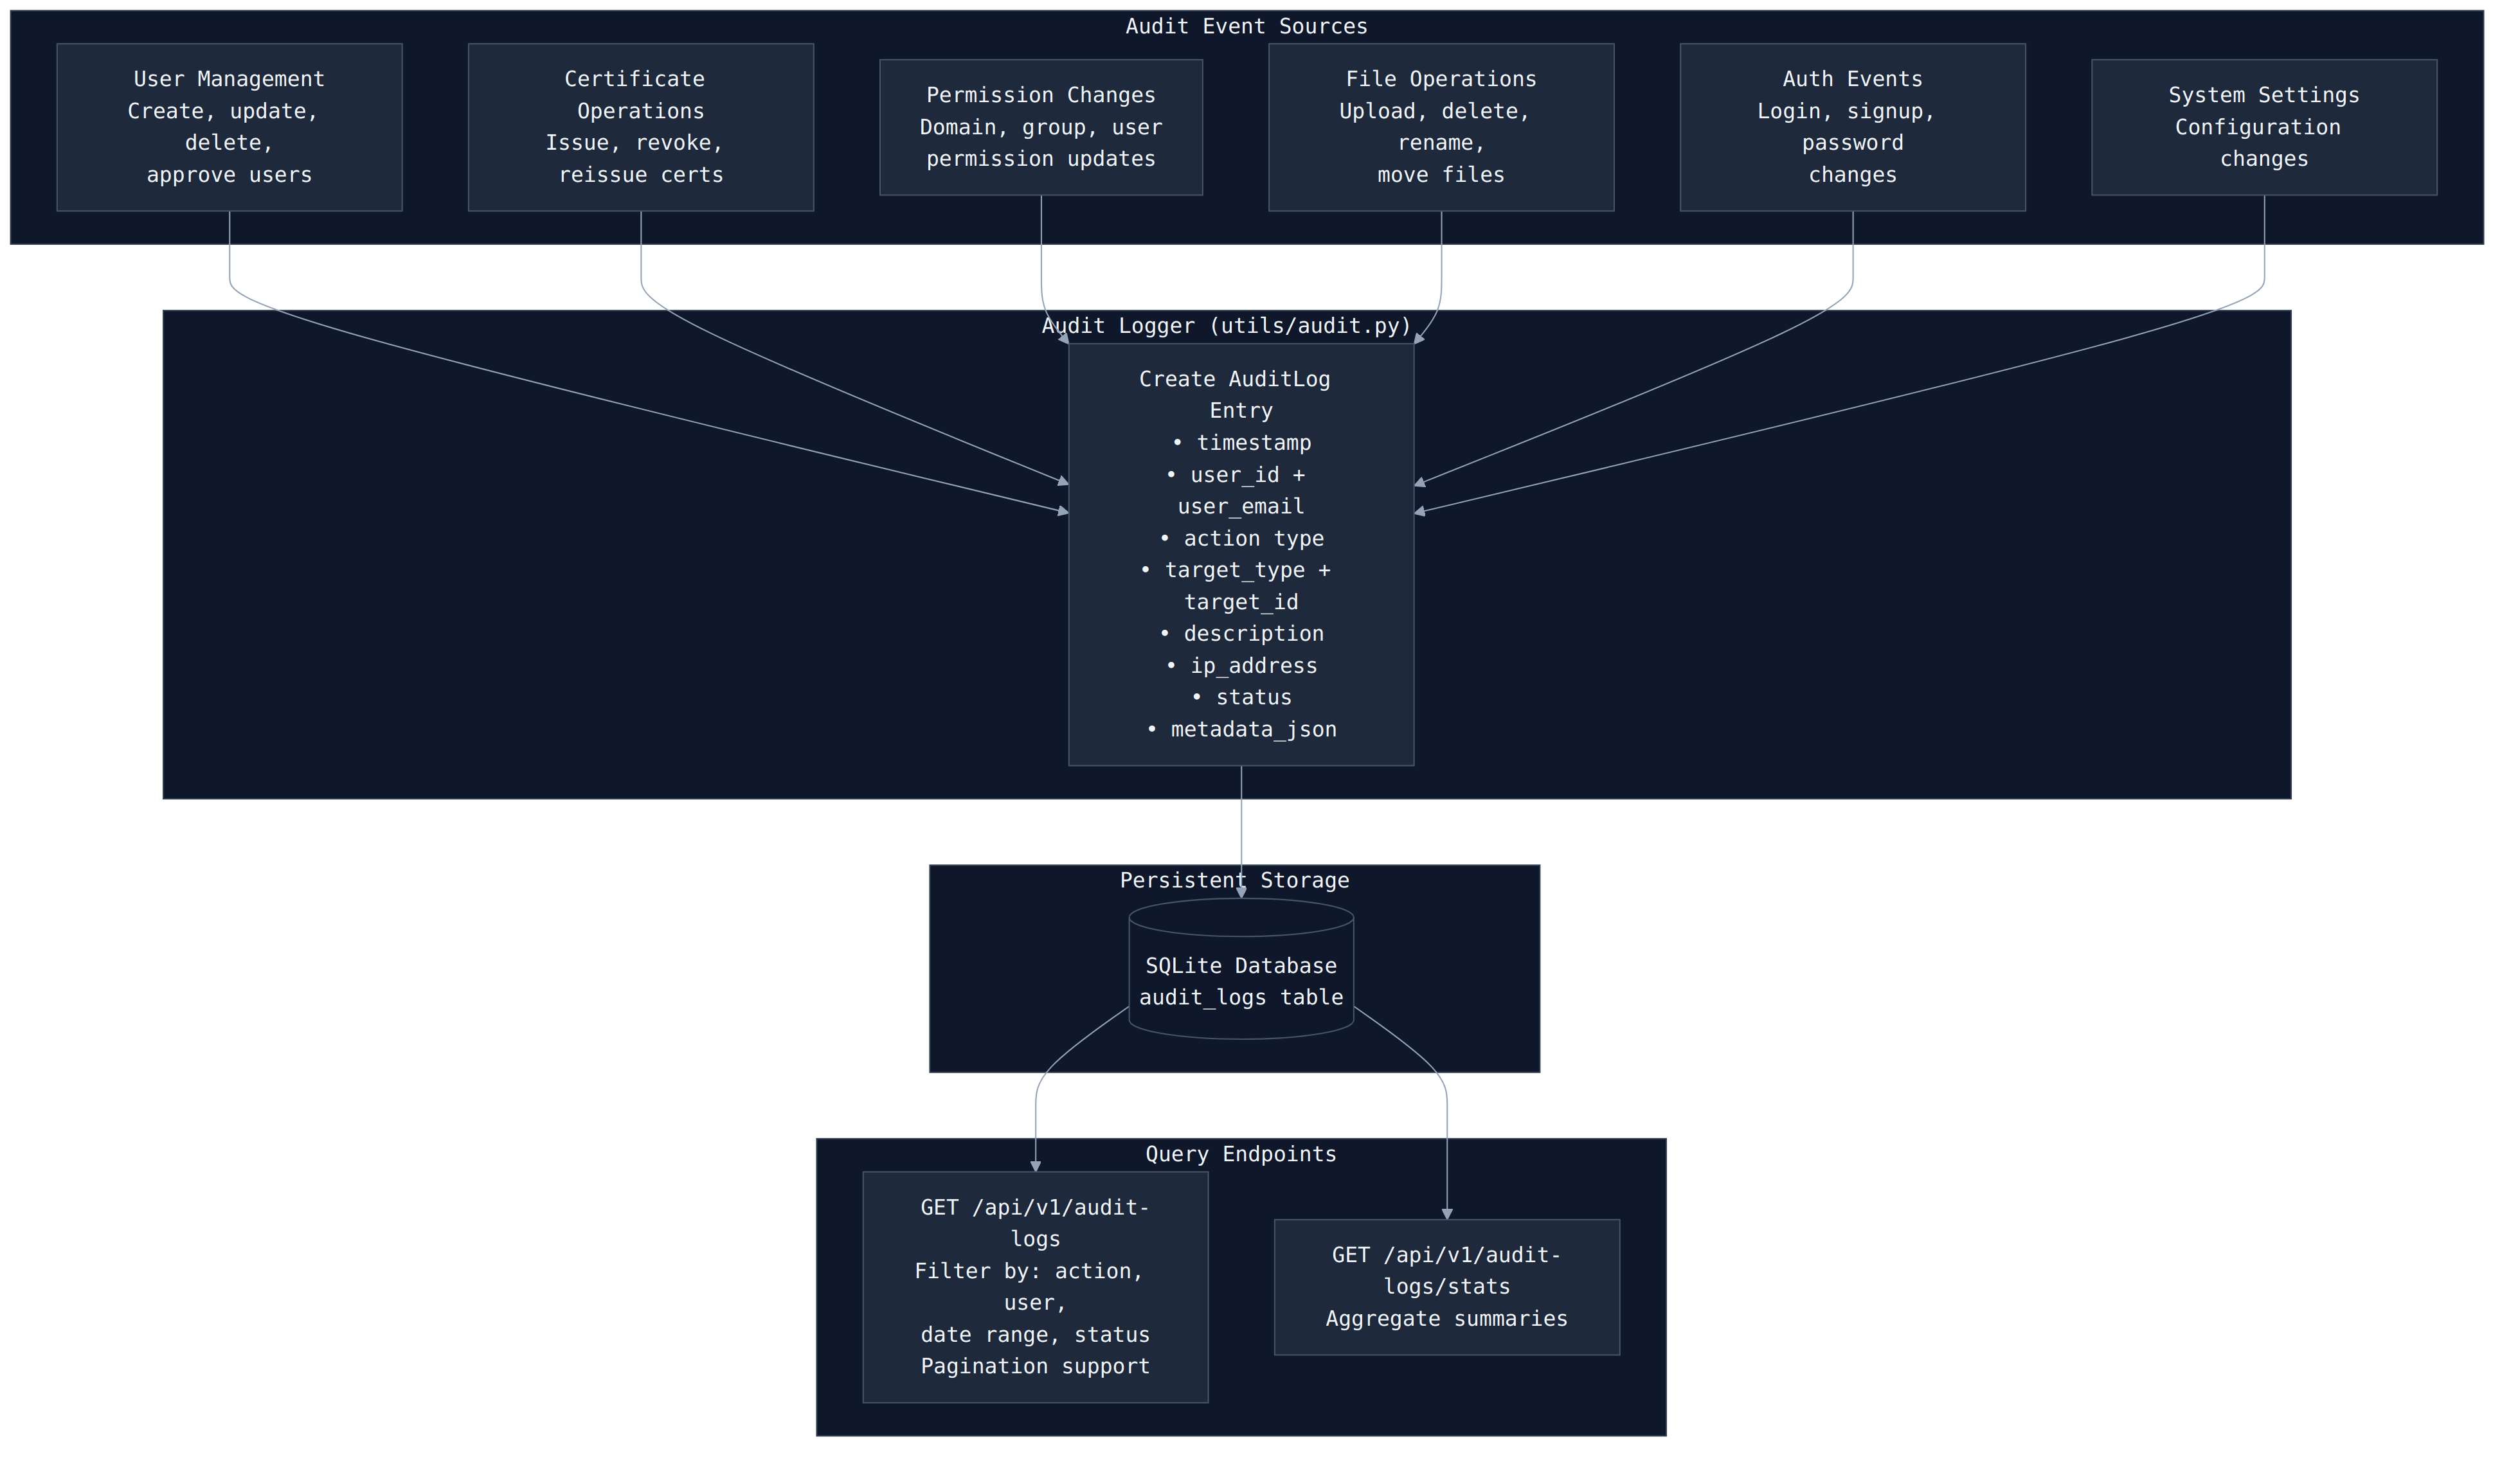
\includegraphics[width=\linewidth]{../diagrams/png/10-audit-logging.png}
% \end{textblock}

% -- Validation --
\begin{textblock}{0.29}(0.684, 0.17)
  \setlength{\baselineskip}{28pt}\setlength{\parskip}{6pt}%
  \pillhead{Validation}\vspace{18pt}\par
  {\fontsize{28}{36}\selectfont\setlength{\baselineskip}{38pt}%
    TerraCrate is validated through automated testing, static analysis, and security evaluation. The backend has 105 unit tests covering authentication, permission resolution, certificate lifecycle, and path traversal prevention, with security-critical invariants explicitly verified: token expiry, deny override logic, and CN mismatch triggered revocation.
The frontend enforces quality through ESLint, TypeScript strict mode, and Vite build verification. A GitHub Actions pipeline enforces all checks on every push before code reaches the main branch.
Security was evaluated against threats inherent to an untrusted wireless environment. mTLS provides replay and session hijacking resistance, bcrypt with short-lived JWTs limits credential exposure, and the CRL ensures immediate access termination on revocation. All administrative actions are captured in a queryable audit log supporting forensics and access accountability.\par}
\end{textblock}

% -- Conclusion --
\begin{textblock}{0.29}(0.684, 0.56)
  \setlength{\baselineskip}{28pt}\setlength{\parskip}{6pt}%
  \pillhead{Conclusion}\vspace{18pt}\par
  {\fontsize{28}{36}\selectfont\setlength{\baselineskip}{38pt}%
    TerraCrate delivers a secure, portable, self-hosted file sharing system that operates
    entirely without cloud infrastructure. By delegating mTLS verification to Nginx, the
    system achieves cryptographic mutual authentication with no client-side software
    beyond a standard browser. The three-tier permission model, automated certificate
    lifecycle management, mDNS discovery, and comprehensive audit logging together
    satisfy all core requirements defined by the client. Future work includes clustered deployment, SMB filesystem access, peer-to-peer synchronization, attribute-based encryption, and anomaly detection on access logs.\par}
\end{textblock}

% -- Acknowledgements --
\begin{textblock}{0.29}(0.684, 0.845)
  \setlength{\baselineskip}{28pt}\setlength{\parskip}{6pt}%
  \pillhead{Acknowledgements}\vspace{18pt}\par
  {\fontsize{28}{36}\selectfont\setlength{\baselineskip}{38pt}%
    The team would like to thank Dr.\ Konstantinos Kolias proposing the project and providing guidance
    throughout the design process.\par}
\end{textblock}

\end{frame}
\end{document}